\documentclass[12pt]{article}
\usepackage{text_style}
\usepackage{mathabx}%$\Mars \Venus$
\title{Diffusion of linear operators}
\author{IA pour la Science}
\date{24 June 2026}
\begin{document}
\maketitle

\section*{Problem statement for Diffusion of linear operators}

There given a collection of pairs $(\bD, \bZ)$ with the dataset $\bD=\{\bx\}$ and the corresponding causal graph $\bZ$.
The elements of the vector $\bx$ is generated by the random variables $X_1,\dots,X_n$ according to some unknown probabilistic structural model.
The linear operator $\bW$ maps a sample $\bx$ to its reconstruction $\hat\bx$.

So $\bZ$ is the $n\times n$ binary matrix that corresponds to $\bW$, the $n\times n$ matrix of the linear operator.

The adjacency matrix $\bZ$ corresponds to the graph $G(V,E)$ with the nodes $V=\{X_1,\dots,X_n\}$ and the edges $E=\{(X_i,X_j)\mid Z_{ij}=1\}$.
Denote the corresponding Structural Causal Model (SCM) as $f_G(\bW,\bx)$.
For this paper fix the structure of a model
\[
     \boldsymbol{0} = \bW\T\bx.
\]
The linear operator that maps $\bx\mapsto\boldsymbol{0}$ corresponds to the matrix of parameters $\bW$.
This matrix is generated from the normal distribution%
\footnote{Generalized Linear Models by J.\,A. Nelder and R.\,W.\,M. Wedderburn, 1972.}
subject to its columns
\[
    \bW = \begin{bmatrix}
        \bw_1 & \bw_2 & \dots & \bw_n
    \end{bmatrix}
    \qquad\text{where}\qquad\bw \sim \cN(\bmu, \bA).
\]
The following assumptions are made:
\begin{enumerate}
    \item The dot product $\bw\T\bA\bx$ define a Riemannian metric on the space of the model parameters $\bw$.
    It holds is the PSD matrix $\bA$ is a metric tensor, non-singular.
    \item The matrix $\bW$ is sparse because the corresponding graph $G$ is sparse.
    So the item above should be statistically tested.
    \item Probably, the representation of the SCM model in the form
    \[
      \boldsymbol{0} = \bW\T\underline{\bA} \bx,
      %\underbrace{\boldsymbol{0}}_{n\times 1} = \underbrace{\bW\T}_{n\times n}\underbrace{\underline{\bA}}_{n\times n\times n} \underbrace{\bx}_{n\times 1},
    \]
    where $\underline{\bA}$ is a tree-way tensor for a quadratic form $\bw\T\bA\bx$ delivers a better quality of the causality reconstruction.
\end{enumerate}

Along with the dataset $\bD$ and the corresponding causal graph $\bZ$ we have a prior distribution $p(\bZ\mid \bD)$.

Formulate the reconstruction problem.
Find the matrix $\bZ$ along with the matrix of the optimal parameters $\hat{\bW}$ and its covariance matrices $\underline{\bA}$
so that the dataset $\bD$ brings the (approximate) kernel to the linear system
\[
    \ker(\bW) =  \{\bD \ni \bx : \| \bW\T\bx \|^2_2 \to \min \}.
\]
Note that the kernel of the linear operator $\bW$ is a subspace of the observable data $\bD$.
Note the singularity of the matrix $\bW$ is a necessary condition for the existence of the kernel.
Note that singular values decomposition of the matrix $\bW$
\[
    \bW = \bU \bLam \bV\T
\]
provides a basis of the kernel.

%$\mars or \venus$.

Denote $d = \dim(\ker(\bW))$.

The algorithm of the causal graph reconstruction
Get the pair $(\bD,\bZ)$ from the collection and set them as $(\bD_0,\bZ_0)$.
Run for $t=0,\dots,T$
\begin{enumerate}
    \item Sample the matrix $\bZ$.
    \item Tune the matrix $\bW$.
    \item Ensure that $d_{t+1}\leq d_t$ with some probability.
    \item Compute the covariance matrix $\bA$ of the model parameters $\bW$. How $X\T X$?
    \item Select some elements for do-intervention.
    \item Generate the do-intervention dataset $\doc(\bD)$.
    \item Compute $\bW\prim,\bA\prim$.
    \item Compute the KL divergence $\KL{p(\bW\prim\mid \bA\prim)}{p(\bW\mid \bA)}$.
    \item If $\KL{}{}$ is statistically significant, then update the model parameters $\bW\to\bW\prim$ and $\bA\to\bA\prim$.
    \item Make the new dataset $\bD_t\to\bD_{t+1}$.
    \item If $\KL{}{}$ is statistically significant, then update the model structure $\bZ\to\bZ\prim$.
    \item Move $t$ to the next step.
\end{enumerate}

make a simple example for one dot product

use the Katrutsa paper


The genetic version of the algorithm.










\end{document}

$P(X_1,\dots,X_n)$ is the distribution of the observable data.
Its approximation is given by the Gaussian Process Regression model
\[
p(\bx \mid f_\text{gp})
\]
on the dataset~
\[\{\bx_i\in\mathbb{R}^n\}.\]
It is indexed by some function of the time and space $(t,s)\mapsto i$.

\subsection*{A model from the family of universal approximators}
For a sample $\bx$ and its reconstruction $\hat\bx$ the likelihood function provided a universal model~$f_\text{nn}(\bth,\bx)$ is
\[p(\bx\mid f_\text{nn}, \bth).\]
Without the a priori information about the model parameters~$\bth$ the corresponding loss function is
\[
\loss(\bth) = -\log p(\bx\mid f_\text{nn}, \bth) = (\hat{\bx} - \bx)\T \mathbf{B}^{-1}(\hat{\bx} - \bx).% + (\bth - \boldsymbol{\mu})\T \mathbf{A}^{-1}(\bth - \boldsymbol{\mu}),
    \]
The matrix $\mathbf{B}$ is the covariance of the reconstruction error.
This matrix in some statements depends on the index~$i$.
This model as a parametric one has a structure to make a distillation to the causal graph
\[
f_\text{nn}(\bth, \bx)  \overset{\text{extract}}{\longrightarrow} \bZ_\text{nn} \overset{\text{dist}}{\longrightarrow}  \bZ.
\]

\subsection*{An SCM we have to forecast}
A structural causal model
\[
    \hat{\bx} = f_G(\bw,\bx) \in\mathcal{F}_\text{scn}
\]
has a structure~$\bZ$ and its probabilistic representation $\bGam$.
The elements of the matrix~$\bGam$ are the probabilities of the causal relationships between the elements of the model structure~$f_G$.
The matrix~$\bZ$ is the adjacency matrix of the causal graph, the binary representation of~$\bGam$.

\medskip
Note: \emph{we suppose that SCM does not fit the whole $(s,t)$-data but a local part of it.
So we also call SCM a local model~$f_G$, in contrast to the universal model~$f_\text{nn}$.}

\subsection*{A foundational model to forecast the SCM}
There given pairs a sample $\bx_i$ and the corresponding SCM~$f_G$ with its structure $\{\bZ_i\}$.
Call the set of pairs
\[(\bx_i, \bZ_i), \quad i\in\cB
\]
a collection of the SCM forecasting.
This collection $\cB$ shows one case of mathematical modeling that results in an interpretable model~$f_G$.
This model fits samples $\bx_i$ from some local data~$i\in\cB$.

Call a model that forecasts an SCM $\mathcal{F}$ a \emph{foundational model}
\[
f_\text{ai}: \bx_\cB \mapsto f_G \in \mathcal{F}.
\]
The SCM is a parametric model
\[
    f_G = f_G (\bw,\bx) \quad\text{with the parameters}\quad \hat{\bw} = \arg\min_{\bw} \loss(\bw).
\]
The foundational model returns not the SCM~$f_G(\hat{\bw},\bx)$ itself,
but only a probabilities~$\bGam$ on the structure~$\bZ$.
So we rewrite the previous definition as
\[
f_\text{ai}: \bx_\cB \mapsto \bGam.
\]

\medskip
Note: \emph{Since a case of mathematical modeling, call it $\cB$ has a history of requests to the foundational model,
    the next information is available for it:
\begin{enumerate}[1)]
    \item the optimal parameters $\bw$ along with $\bZ, \bGam$ for the SCM $f_G$,
    \item the prior probabilities of the model parameters $p(f_G)$ or all models in the family $\mathcal{F}$,
    \item the other information about the case of mathematical modeling $\cB$ that is relevant for the forecasting of the SCM.
\end{enumerate}}

\subsection*{The Integer Linear Programming for the causal graph selection}
The matrix $\bGam$ comes along with the descriptions of its nodes $X_1,\dots,X_n$, and the probabilities.
The SCM $f_G$ is defined by the graph $G=(\bZ,X)$ by solving
\[
  \text{ILP}(\bGam,P_X) \to \bZ \to f_G.
\]

\subsection*{The evidence of the SCM}
A probabilistic description~$\bGam$ of a model $f_G$ from the class of \emph{admissible models} $\mathcal{F}$ is generated from a parametric distribution
\[
    \bGam \sim \text{Dir}(\bpi) \quad\text{generated by MCMC}\quad f_\text{mh}(\bpi),
\]
here the lowercase letters mean Metropolis-Hastings Algorithm for MCMC.
(A simple genetic algorithm may bring some decent results, too).
This distribution provides a probabilistic space for the similar models.
See the document on \emph{Multimodeling}.

The model $f_G$ and the corresponding graph has its likelihood
\[
    p(\bx|f_G).
\]
See the document on \emph{Causal graph likelihood}.

\medskip
Note: \emph{Two-level bayesian inference introduces the probability of the SCM parameters on the first level.
And the probability of the model on the second level is:
    \begin{enumerate}[1)]
    \item the prior of the SCM is delivered by the generative model $f_\text{mh}$
    \item the likelihood of the SCM is delivered by the forecasting model $f_\text{ai}$.
\end{enumerate}}

\subsection*{The criterion of causality}
The parameters of the model $f_G$ has their covariance matrix.
The prior of the model parameters is
\[
    - \ln p(\bw|f_g) = (\bw - \bmu)^{\mathsf{T}} \bA^{-1} (\bw - \bmu).
\]
The algorithm of the Bayesian hyperparameters $(\bmu, \bA)$ estimation
(and their connection between the causality)
is described in the document on \emph{parameter analysis}.

\subsection*{A model for the intervention}
See the document on the \emph{intervention strategy}.

\end{document}

\section{Functional diagram of the model forecasting}
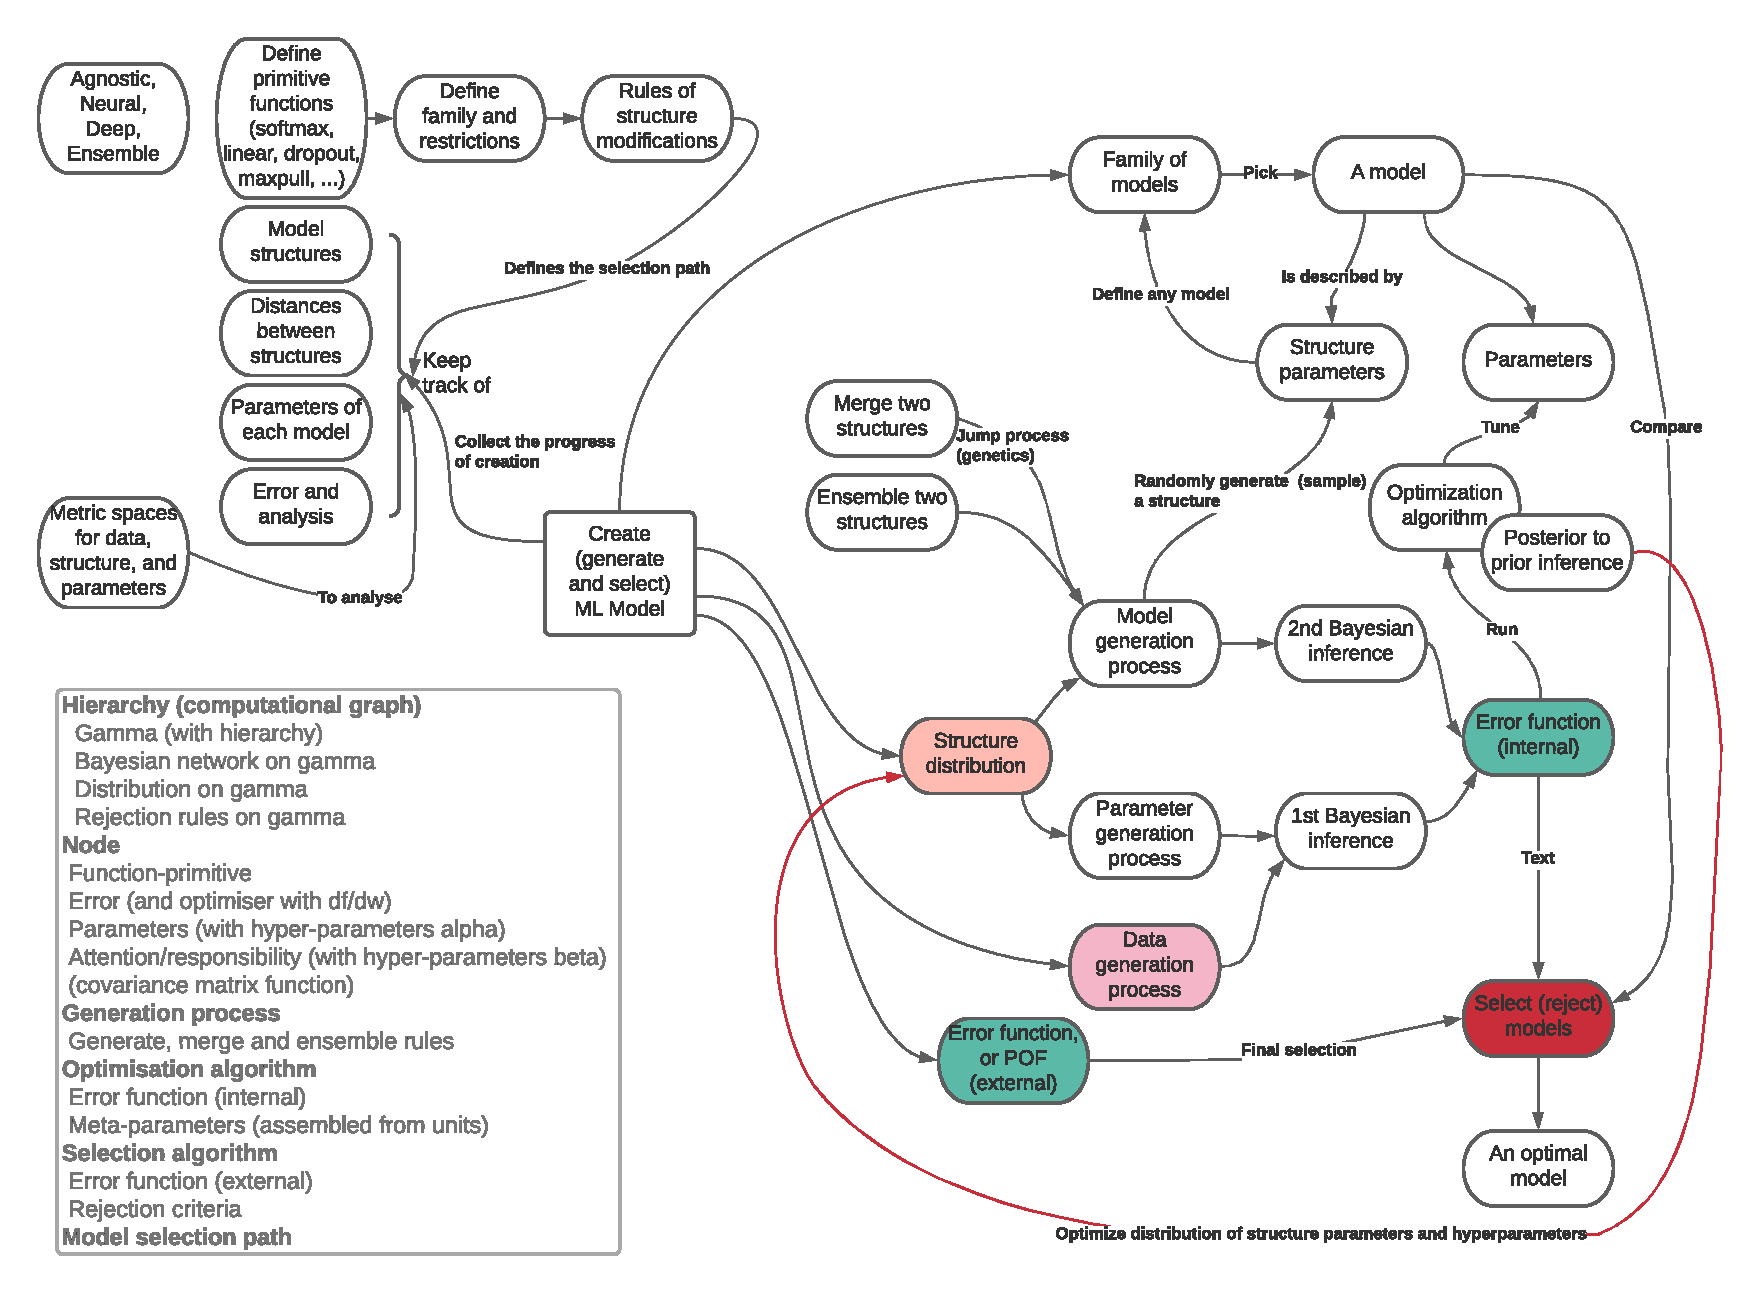
\includegraphics[width=\textwidth]{intro_structure_learning_map.pdf}

\section{Generall problem statement in multimodeling}
\includegraphics[width=\textwidth]{tmp/fig_multi_mod_1}

\section{When do we need a multimodel}
\includegraphics[width=\textwidth]{tmp/fig_multi_mod_2}

\section{Model comparison hypotheses}
\includegraphics[width=\textwidth]{tmp/fig_multi_mod_3}

\section{Proposed statement of the model comparison}
\includegraphics[width=\textwidth]{tmp/fig_multi_mod_4}

\section{Explicit form of $s(g_1,g_2)$ for a pair of normal distributions}
\includegraphics[width=\textwidth]{tmp/fig_multi_mod_5}

\section{Mixture of experts as a multimodel}
\includegraphics[width=\textwidth]{tmp/fig_multi_mod_6}

\section{Similarity of models in a multimodel}
\includegraphics[width=\textwidth]{tmp/fig_multi_mod_7}

\section{Model comparison issues}
\includegraphics[width=\textwidth]{tmp/fig_multi_mod_8}

\section{Requirements to the similarity function}
\includegraphics[width=\textwidth]{tmp/fig_multi_mod_9}
\end{document}









\documentclass[12pt]{article}
\usepackage[utf8]{inputenc}
\usepackage[T1]{fontenc}
\usepackage{amsmath,amsfonts,amssymb}
\usepackage{enumerate}
\usepackage{graphicx}
\usepackage{a4wide}
\usepackage{xypic}
\usepackage{mathtools}
\newcommand\indep{\mathrel{\perp\mspace{-10mu}\perp}}
\newcommand\nindep{\mathrel{\mathrlap{\not}\mspace{-7mu}\indep}}
\newcommand{\KL}[2]{D_{\mathrm{KL}}\!\left(#1 \,\middle\|\, #2\right)}
\newcommand{\doop}{\mathrm{do}}
\newcommand{\Anc}{\mathrm{Anc}}
\newcommand{\Pa}{\mathrm{Pa}}
%\newcommand{\argmax}{\mathop{\arg\max}}
\newcommand{\argmax}{\operatorname*{arg\,max}\limits}
\newcommand{\T}{^{\mathsf{T}}}
\newcommand{\eL}{\mathcal{L}}
\newcommand{\doc}{\mathrm{do}}
\newcommand{\bW}{\mathbf{W}}
\newcommand{\ba}{\mathbf{a}}
\newcommand{\bb}{\mathbf{b}}
\newcommand{\bx}{\mathbf{x}}
\newcommand{\bw}{\mathbf{w}}
\newcommand{\by}{\mathbf{y}}
\newcommand{\bz}{\mathbf{z}}
\newcommand{\bmu}{\boldsymbol{\mu}}
\newcommand{\bSig}{\boldsymbol{\Sigma}}
\newcommand{\bA}{\mathbf{A}}
\newcommand{\cA}{\mathcal{A}}
\newcommand{\cB}{\mathcal{B}}
\newcommand{\loss}{\mathcal{L}}
\newcommand{\cN}{\mathcal{N}}

\title{Causal discovery with parameter analysis}
\author{IA pour la Science}
\date{25 March 2026}
\begin{document}
%\maketitle
%\begin{abstract}
%    abstract
%\end{abstract}
%\section{Introduction}
\section*{Test the model structure with do-generated dataset}
There given an observation data $(\bx,\by)$ and a model $f=f(\bx; \bw, \cA)\mapsto \by$.
There given the model parameters $\hat{\bw}$ and the model structure $\hat{\cA}$  so that three loss functions holds
\begin{enumerate}[1)]
\item inference loss $\loss\bigl(f(\bx)\bigr)\to \mathop{\min}\limits_{\bw,\cA}$,
\item reconstruction loss  $\loss\bigl(f^{-1}(\by)\bigr)\to \mathop{\min}\limits_{\bw,\cA}$.
\end{enumerate}
They are obtained by the backpropagation algorithm. The distribution of the parameters $p(\bw\mid \bx,\by,\cA)$ is estimated during their optimization. The structure~$\cA\in\mathbb{B}^n$ (for deep networks a hypergraph on its elements is defined). 

\medskip
One has to find the optimal test set $\{\doc(\bx,\by)\}$ that maximizes the distance between the structure $\rho(\cA,\cA_\doc) = \exp\bigl(-|\cA-\cA_\doc|\bigr)$ element-wise for each test case $\{\doc(\bx,\by)\}_{\cB_i}$:
\[
\sum\limits_{i}\rho(\cA,\cA_\doc\bigl(\cB_i)\bigr) \to\mathop{\max}\limits_{\{\doc(\bx,\by)\}}.
\]
In the other words, one has to generate a data, so that for each sample set indexed~$\cB_i\}$ there is a statistically significant change in one element of the model structure~$\cA$ (or a vertex of the structure hypergraph).

Suppose the generated data $\doc(\bx,\by)$ must be similar to the distribution of the observable data for both distributions 
$p(Y\mid X=\bx)$ and $p(X\mid Y=\by)$. (Best option: one can select from the observation data set a subset to test such that it tests an element of model structure.)

\medskip
The data generation procedure uses the perturbation of parameters. For simplicity assume a perturbation of a single parameter~$w_i$ with the distribution $p(\hat{\bw}) = \cN(\hat{\bw}, \hat{\bA})$  for some subset of the model parameters.
Denote~$w_\doc = w+\delta$, where the value of $\delta \gg \frac{\varsigma}{\sqrt{n}}$ is chosen so that the Student t-test detects statistically significant difference. 
The data generation algorithm is the following:
\begin{enumerate}[1)]
\item select an $i$-th element of the model structure~$\cA$,
\item sample the parameter $w_i$ so that $\doc(w_i) = w_i+\delta$,
\item denote the indexes of the samples by $\cB_i$,
\item with the backpropagation generate $\bx_\doc$ samples, 
\item with the inference (propagation) generate $\by_\doc$ samples, 
\item gather the generated test dataset $\{\do(\bx,\by)\}_{\cB_i}$,
\item to use to test the model structure~$\cA$ and ensure that 
\[
\doc(\bx,\by) \to \cA_\doc \quad\text{for each}\quad i.
\]
\end{enumerate}

Note that both backpropagation and inference require data from the observation set to compute the generated data. Assume that these data are expected values (given time and space for spatial-time data).

Variants of samples in the generated data. 
\begin{enumerate}
\item Generation of an element delivers outlines in the data, $ \doc(\bx,by) \sim p(X,Y)$ does not hold.
\item Generation of an element delivers expected data.
\end{enumerate}

The procedure of usage of the generated data to eliminate statistically non-relevant elements from the model structure~$\cA$:
\begin{enumerate}[1)]
\item estimate the model parameters $p(\bw\mid \bx,\by,\cA)$,
\item sample the do-parameters $p(\bw_\doc)$ assuming them as the prior distribution,
\item obtain generated dataset $\doc(\bx,\by)$,
\item estimate the loss~$\loss\bigl(f(\bx)\bigr)$ for inference and reconstruction~ $\loss\bigl(f^{-1}f(\by)\bigr)$,
\item find the unused elements of the model structure~$\cA$ such that 
\[
\cA_\doc = \mathop{\arg\min}\limits_{\{\doc(\bx,\by)\}} \lambda\loss\bigl(f(\bx)\bigr) + (1-\lambda)\loss\bigl(f^{-1}f(\by)\bigr).
\]
\end{enumerate}
For the selection of model structure procedure the complexity $\mathcal{O}(2^\cA)$ drops to lesser than $\mathcal{O}(\cA)$, since the only procedure we need is to generate the model parameters~$\bw_\doc$.
 





\maketitle
\section{The main algorithm}

There given a sample set of interventions
\[
    V_\doop = \{\doop(V = v_0), \doop(V = v_1), \dots \},
\]
where~$v_i$ (is a) set of all nodes.

\begin{enumerate}%[1)]
    \item Assume we have samples of $V_\doop$ (with <<a>> distribution) and the variables for any $V\in v$
    \[
        S_1^v,\dots S_n^v.
    \]
    \item For any $y \in V$, compute $\Anc(y)$ by:
    \[
        \Anc(y) = \{ v, y \nindep V_\doop \}.
    \]
    \item For each, $\forall\, Y \in V, \forall\, x \in \Anc(y)$:
    \begin{enumerate}%[1)]
        \item estimate $w_i^{yx} = \argmax_w P(y\mid X_\doop; w)$,
        $ 1 \leq i \leq n$ and obtain $\hat{w}_1^{yx}, \dots, \hat{w}_n^{yx}$,
        where $P(y\mid X_\doop; w)$ in the probability of $Y$ from $\Anc(Y)$ based on all samples, assessed with~$X$;
        \item compute $\hat{\bmu}^{yx}$ and  $\hat{\bSig}^{yx}$ from $\hat{w}_1^{yx}, \dots, \hat{w}_n^{yx}$;
        \item compute $\KL{p(w; \hat{\bmu}, \hat{\bSig})}{p(w; \hat{\bmu}^{xy}, \hat{\bSig}^{xy})}$;
        \item if $\KL{}{} \geq 0$, $x \in p_a(Y)$.
    \end{enumerate}
\end{enumerate}

\paragraph{The first variant}
\[
X_\doop \{ \doop (X = x_0), \doop (X=x_1), \dots \};
\]

$V_i$ set of all nodes

(a) If $X_\doop \nindep Y$, then $X \in \Anc(Y)$

\begin{itemize}
    \item If there exists $\doop(Z)$, where $Z = V\setminus X$, s.t. $X\indep Y \mid \doop(Z)$, then $X\notin Pa(Y)$.
    \item Otherwise, $X\in\Pa(Y)$ $\to$ impossible in practice
\end{itemize}

(b) With (a) we can compute the ancestors of all variables , e.q.
\[
\begin{aligned}
    \Anc(Y) = \{V,Z,X,V\},  & \Anc(X) = \{V\}           & => & \Pa(X) = \{V\} \\
    \Anc(V) = \{X,V\},      & \Anc(V) = \{\emptyset\}   & => & \Pa(V) = \{\emptyset\} \\
    \Anc(Z) = \{X,V\},      &                           & => & ? Z \indep X \mid V
\end{aligned}
\]

\includegraphics[width=.4\textwidth]{../temporary/tab_DAG1}
\includegraphics[width=.4\textwidth]{../temporary/tab_DAG2}

\section{Classification as a criterion of causal disturbance}
\begin{itemize}
    \item Set a tests for the causal disturbance: $X$ and $X=\bx_0$.
    \item Train a classifier to distinguish between the parameter distribution
    \item The distribution of the model parameters are the features.
    \item Maximize the gap between two classes
\end{itemize}
%+++++++++++++++++++++++++++++++++++++++++
%+++++++++++++++++++++++++++++++++++++++++
\iffalse

%+++++++++++++++++++++++++++++++++++++++++
... some notes for the presentation
%+++++++++++++++++++++++++++++++++++++++++
\fi
%+++++++++++++++++++++++++++++++++++++++++
%+++++++++++++++++++++++++++++++++++++++++
%\begin{gather*}
%    X \perp\!\!\!\perp Y \mid Z\\
%    X \indep_C Y \mid Z\\
%    \KL{P}{Q}\\
%\end{gather*}
%+++++++++++++++++++++++++++++++++++++++++

\maketitle

\section*{Introduction}
The goal of this document is to describe the target function of the causal graph.

We treat the algorithm PCGCE in the paper \emph{Extended summary graphs (ESG)} belongs to
class of the exhaustive search algorithms.
So to an optimal causal graph we make no difference between
\begin{enumerate}[1)]
\item exhaustive printing or combinatorial algorithms,
\item gradient-based algorithms including algorithms with relaxations,
\item  zero-gradient algorithms.
\end{enumerate}
The only thing we expect its result is a causal graph, optimal according to this criterion.

\medskip
The model structure includes:
\begin{enumerate}[1)]
\item the time is continuous $\frac{dx}{dt}=f(x,t)$ (basic: discrete with $\Delta t=1$),
\item the time series $X, Y, Z$ has a spacial structure $\frac{dx}{dx} = g(x,s)$ (basic: scalar-valued),
\item there is no limitations of the time as in the ESG,
\item the model is linear in the latent space (basic: linear in the observable space),
\item the latent space represent a spectrum of the observable domain.
\end{enumerate}

\medskip
The graph structure:
\begin{enumerate}[1)]
\item the graph is a bipartite graph between the observable and the latent,
\item the direct graph is isomorphic to the reverse graph,
\item the causal graph is in the hypergraph that groups the variables or the time.
\end{enumerate}
The time structure for the convolutional model $\int_{\tau=0}^T f(\tau)h(t-\tau)d\tau $

\medskip
The causal graph $G=G(t)$ is a time series.
We suppose either:
\begin{enumerate}[1)]
\item it is stationary fot all $t$,
\item it is stationary for $t\geq T$ for with the period $T$,
\item it is non-stationary but with rejection to discover its structure.
\end{enumerate}

\section{Appendix. Natural Gradient Descent}
The natural gradient descent is a method to optimize the model parameters $\theta$ by estimating the distribution
\[
    p(\theta) \propto \exp(-\eL(\theta))
\]
where $\eL(\theta)$ is the loss function of the model.
The natural gradient descent is defined as
\[
    \theta_{t+1} = \theta_t - \eta F^{-1}
\]
where $F$ is the Fisher information matrix of the model parameters $\theta$.

\subsection*{Fisher Metric and Natural Gradient}

When working with probabilistic models, we can use a metric that is more natural for probability distributions: the Kullback--Leibler (KL) divergence. Suppose we have a likelihood model
\[
p(x \mid \theta),
\]
where \(x\) denotes fixed data and \(\theta\) is a parameter vector.

Let \(\theta_t\) denote the current parameter values, and suppose we wish to find updated parameters \(\theta_{t+1}\). Under the natural gradient framework, this is done by solving the following optimization problem:
\[
\theta_{t+1}
=
\arg\min_{\theta}
\left[
f(\theta_t)
+
\nabla f(\theta_t)^\top (\theta - \theta_t)
+
D_{\mathrm{KL}}\!\left(
p(x \mid \theta)
\;\|\;
p(x \mid \theta_t)
\right)
\right].
\]

In general, this minimization problem is intractable. However, the KL divergence can be approximated locally using a second-order Taylor expansion. This expansion yields the Fisher information matrix \(F\), which captures the local curvature of the statistical manifold. In particular, around \(\theta_t\), we have
\[
D_{\mathrm{KL}}\!\left(
p(x \mid \theta)
\;\|\;
p(x \mid \theta_t)
\right)
\;\approx\;
\frac{1}{2}
(\theta - \theta_t)^\top
F
(\theta - \theta_t),
\]
where the Fisher information matrix is defined as
\[
F
=
\mathbb{E}_{x \sim p(x \mid \theta)}
\left[
\bigl( \nabla_\theta \log p(x \mid \theta) \bigr)
\bigl( \nabla_\theta \log p(x \mid \theta) \bigr)^\top
\right].
\]

The Fisher information matrix therefore encodes the curvature of the likelihood-based loss function in parameter space. Using this approximation, the resulting natural gradient update rule becomes
\[
\theta_{t+1}
=
\theta_t
-
\gamma
F^{-1}
\nabla f(\theta_t),
\]
where \(\gamma > 0\) is the learning rate.

\subsection*{Natural Gradient from an Information-Geometric Perspective}

Consider a parametric family of probability distributions
\[
\mathcal{M} = \{ p(x \mid \theta) \mid \theta \in \Theta \subset \mathbb{R}^d \},
\]
which forms a smooth statistical manifold \(\mathcal{M}\). Each parameter vector \(\theta\) corresponds to a point on this manifold, and the coordinate system \(\theta\) is generally non-Euclidean.

The natural notion of distance between nearby probability distributions on \(\mathcal{M}\) is given by the Kullback--Leibler divergence. For two infinitesimally close distributions \(p(x \mid \theta)\) and \(p(x \mid \theta + d\theta)\), the KL divergence admits the second-order expansion
\[
D_{\mathrm{KL}}\!\left(
p(x \mid \theta + d\theta)
\;\|\;
p(x \mid \theta)
\right)
=
\frac{1}{2}
d\theta^\top
G(\theta)
d\theta
+
o(\|d\theta\|^2),
\]
where
\[
G(\theta)
=
\mathbb{E}_{x \sim p(x \mid \theta)}
\left[
\bigl( \nabla_\theta \log p(x \mid \theta) \bigr)
\bigl( \nabla_\theta \log p(x \mid \theta) \bigr)^\top
\right]
\]
is the **Fisher information metric tensor** on \(\mathcal{M}\).

Let \(f(\theta)\) be a smooth objective function defined on the manifold (e.g., the negative log-likelihood or empirical risk). Given the current point \(\theta_t \in \mathcal{M}\), we seek a new point \(\theta_{t+1}\) by minimizing a first-order approximation of \(f\) subject to a constraint on the geodesic distance induced by the Fisher metric. This leads to the optimization problem
\[
\theta_{t+1}
=
\arg\min_{\theta}
\left\{
f(\theta_t)
+
\nabla f(\theta_t)^\top (\theta - \theta_t)
\;\middle|\;
D_{\mathrm{KL}}\!\left(
p(x \mid \theta)
\;\|\;
p(x \mid \theta_t)
\right)
\le \epsilon
\right\}.
\]

Using the local quadratic approximation of the KL divergence, this constrained problem reduces to minimizing the linearized objective under a Riemannian norm constraint. The solution is given by a step in the direction of the **natural gradient**, defined as
\[
\widetilde{\nabla} f(\theta)
=
G(\theta)^{-1}
\nabla f(\theta).
\]

Accordingly, the natural gradient descent update takes the form
\[
\theta_{t+1}
=
\theta_t
-
\gamma
\widetilde{\nabla} f(\theta_t)
=
\theta_t
-
\gamma
G(\theta_t)^{-1}
\nabla f(\theta_t),
\]
where \(\gamma > 0\) is the step size.

From an information-geometric standpoint, this update corresponds to moving along the direction of steepest descent with respect to the Fisher–Rao Riemannian metric, ensuring invariance under smooth reparameterizations of the statistical manifold.


\newpage
    \section{Second document}

\section*{Introduction}
We construct a Bayesian causal-inference model for multivariate time series.
The goal is to identify a causal relationship between time series given the constructed model.
We suppose that the unknown dynamics generated the observable time series from the latent space.
Here we keep the model simple to expand it for
    1) multimodal time series and control problems,
    2) transformers and large models,
    3) continuous-time dynamical systems and Neural ODE.

\section{Discrete-time linear model}
There given time series $\mathbf{x}_t$ as observations.
The time series are generated by a discrete-time dynamical system in the latent space~$\mathbf{z}_t$ with unknown dynamics:
\begin{equation}\label{eq:linear-model}
    \mathbf{x}_{t+1} = f\bigl(\mathbf{x}_t\bigr)  + \boldsymbol{\zeta}_{t+1},
\end{equation}
where $\boldsymbol{\zeta}_{t}$ is the noise term.
The linear model is
\[
   \mathbf{x}_t = \mathbf{W}\mathbf{x}_{t-1} +\mathbf{b} + \boldsymbol{\zeta}_{t}.
\]
The time series are represented via \emph{delay embedding}.
The matrix of delay vectors for the scalar-valued series~$x_t$ is the Hankel matrix~$\mathbf{X}$.
Let the vector~$\mathbf{x}_{t-1}$ be the first column of the matrix~$\mathbf{X}_{t-1}$.
Each column of the matrix~$X$ contains a point~$\mathbf{x}_t$.
Call~\emph{the phase trajectory} of a dynamical system the sequence~$\{\mathbf{x}_t\}$.
The dimensionality of the model is
\[
    \begin{pmatrix}
        w_{1,1} & w_{1,2} & \cdots & w_{1,N} \\
        w_{2,1} & w_{2,2} & \cdots & w_{2,N} \\
        \vdots  & \vdots  & w_{\kappa,\tau} & \vdots  \\
        w_{K,1} & w_{K,2} & \cdots & w_{K,N}
    \end{pmatrix}
    \underbrace{
    \begin{pmatrix}
        x_{t-1} & x_{t-2} & \cdots & x_{t-(N+T)} \\
        x_{t-2} & x_{t-3} & \cdots & x_{t-(N+T-1)} \\
        \vdots & \vdots & x_{t-\tau} & \vdots \\
        x_{t-N} & x_{t-(N-1)} & \cdots & x_{T}
    \end{pmatrix}}_{\text{Hankel matrix }\mathbf{X}_{t-1}}.
\]
The model parameters are
\[
w_{\kappa,\tau},\;
\tau=1,\dots,K,\;
\kappa=1,\dots,N.
\]
For the vector autoregression model $N=K$.
Otherise suppose $N\gg K$ and call $N$ the original embedding dimension and $K$ the reduced embedding dimension.
The discrete time lag~$\Delta t = 1$ and $T\ni\{1,\dots,t\}$ is the sample size.
For $d$-variate time serires~$\mathbf{x}_t^{(1,\dots,d)}$, the matrix~$\mathbf{X}$ is block-Hankel with $d$ blocks.
The matrix~$\mathbf{W}$ in this case is $(K\times d\cdot N)$.
% TODO include an example with the phase trajectory

\section{State space reconstruction}
Introduce the singular value decomposition of the linear operator in the model~\eqref{eq:linear-model}:
\[
  f=\mathbf{W}\boldsymbol{\Lambda} \mathbf{V}\T.
\]
Denote by~$\mathbf{z}$ the variable in the latent space. It corresponds to the dynamics of the system,

\begin{equation*}
    \xymatrix{
        \mathbf{x} \ar "1,3"^{f} \ar "2,2"_{\mathbf{W}} & ~  & \mathbf{y} \\% \ar "2,2"_{\mathbf{V^\mathsf{T}}}  \\
        ~ & \mathbf{z} \ar "1,3"_{\boldsymbol{\Lambda}\mathbf{V}^\mathsf{T}} & ~ \\
    ~ & t \ar "2,2"^{p(\mathbf{z}|t)} & ~
    }
\end{equation*}
For simplicity omit the time $t$ and the bias~$\mathbf{b}$ in the model~\eqref{eq:linear-model}.
Let the variable~$y$ be the forecast of the time series~$x_t$.
The variable~$\mathbf{z}$ is the projection of the observable~$\mathbf{x}$ onto the low-dimensional latent space.

In the terms of neural networks, this superposition is an encoder and a decoder.
The linear operators $\mathbf{W}$ and $\mathbf{V}$ are the orthogonal and $\boldsymbol{\Lambda}$ is diagonal with positive descending elements.
Each row of the matrix~$W$
\[
\mathbf{W}\mathbf{x} =
    \begin{pmatrix}
        \mathbf{w}_1\T \\ \mathbf{w}_2\T \\ \vdots \\ \mathbf{w}_K\T
    \end{pmatrix} \mathbf{x}
\]
produces an element of a vector~$\mathbf{z}$ in the latent space by the dot product
\[
    z_i = \mathbf{w}_i\T \mathbf{x}.
\]
Call the \emph{embedding} the linear map $\mathbf{z}=\mathbf{W}\mathbf{x}$.

The system dynamics is represented by the generative model~$p(\mathbf{z} \mid t)$.
It approximates the embedding in the latent space with the support $t$.

\section{Maximum a posteriori estimation of the parameters}
The posterior distribution of the model parameters~$\mathbf{w}$ given the data~$\{\mathbf{x}, \mathbf{y}\}$ is
\[
    p(\mathbf{w}|\mathbf{x}, \mathbf{y}) = \frac{p(\mathbf{y}|\mathbf{x}; \mathbf{w}) p(\mathbf{w}|\mathbf{x})}{p(\mathbf{y}|\mathbf{x})}.
\]
The likelihood function is
\[
    p(\mathbf{y}|\mathbf{x}; \mathbf{w}) = \prod_{t=1}^T p(\mathbf{y}_t|\mathbf{x}_t; \mathbf{w}).
\]
The error given the posterior distribution of the parameters is
\[
    \eL(\mathbf{w}) = \frac{1}{2}
    \underbrace{
        (\mathbf{f}-\mathbf{y})\T \mathbf{B}^{-1}(\mathbf{f}-\mathbf{y})
    }_{\text{reconstruction error}}
    + \frac{1}{2}
    \underbrace{
        (\mathbf{w} - \boldsymbol{\mu})\T \mathbf{A}^{-1}(\mathbf{w} - \boldsymbol{\mu})
    }_{\text{error in parameters}}.
\]
Let the matrix $\mathbf{B}=\beta \mathbf{I}$ for the hypothesis that the variance~$\beta$ of the reconstruction error the same in the time segment $(1,\dots,T)$.
The variance~$\beta$ is estimated as empirical distribution from the data over time~$t$.
The covariance~$\mathbf{A}$ and the mean~$\boldsymbol{\mu}$ of the normally-distributed parameters are estimated as empirical distribution from the data.
% TODO Insert an algorithm how to sample the \emph{empirical} parameter distribution (estimate the expectation and variance).

\section{The criterion of causality}
The criterion of the causal relationship between the elements of the model,
we use the Kullback-Leibler divergence between the distributions of the parameters given the intervention~$\doc(\mathbf{x})$:
\[
    \text{KL}\bigl(p(\mathbf{w}|\mathbf{x},\mathbf{y},
    ||
    \,p(\mathbf{w}|\doc(X=\mathbf{x}_0),\mathbf{y}\bigr),\]
where~$\{\mathbf{w}\}=\mathbf{W}$ is the set of the model parameters.
% TODO insert the KL-trick where should be the first and the second argument.
The parameters are maximized according to the maximum a posteriori criterion.

For a linear operator~$\mathbf{W}$, elimination of an edge from a node~$X$,
an element of the vector~$\mathbf{x}_t$,
is equivalent to zeroing the corresponding item~$w_{\kappa,\tau}$.
The node~$X$ corresponds to a column in~$\mathbf{W}$.
Since the parameter~$w$ is a random variable, the following statement holds, see Table~\ref{tab:causal-criterion}.
\begin{table}[hp]
    \label{tab:causal-criterion}
    \caption{The action for a node based on the variance of the parameter~$w$.}
    \begin{tabular}{|l|l|l|l|}
        \hline
        \bf{Expectation} & \bf{Variance} & \bf{Statement} & \bf{Action} \\ \hline \hline
        0       & tends to 0        & Sure that there is no impact  & Remove the node\\
        0       & not tends to 0    & Uncertain about the impact    & Research to remove\\
        not 0   & tends to 0        & Sure that there is an impact  & Assert the node\\
        not 0   & not tends to 0    & The impact must be specified  & Research to assert\\
        any     & large values      & Sure that there is no impact  & Remove the node\\
        \hline
    \end{tabular}
\end{table}

\section{The intervention algorithm}
\begin{enumerate}
    \item One step of back-prop in one layer.
    \item Compute the covariance of the parameters (note the relation between Cov, Hessian and Fisher matrices).
    \item Select a node~$X$ to make an intervention.
    \item Make an intervention $\doc(X=\mathbf{x}_0)$ for a given node.
    \item Compute the KL divergence between the distributions of the parameters with and without intervention.
    \item Remove the intervention and go to step~1 until all nodes are processed.
    \item The causal graph is constructed as a directed graph with edges weighted by the KL divergences.
\end{enumerate}

\section{$\doc(X)$ intervention policy}
For regression or one-class classification, $do(X = x)$ is considered with values of $x$ that lie outside the distribution of the time series at time $t$.
For two-class classification, $do(X = x)$ is considered with values of $x$ equal to the expectation of the opposite class.

What happens after the intervention?
Until the forecasting and reconstruction error remains the same:
\[
    \eL\bigl(p(\mathbf{y}|\mathbf{x}; \mathbf{w})\bigr) = \text{const},
\]
%When the error increases, The model parameters change.
\begin{enumerate}
    \item Until the end of the short-term forecast horizon.
    \item From one of sides, either $X$ or $Z$, we start the intervention.
    \item Start with the parameter of maximum variance of reconstruction error
    \item Then, move to the parameters with lower variance.
    \item Estimate the KL divergence of maximum posterior after each intervention.
    \item Analyse the expectation and the variance of the parameters.
    \item Eliminate the parameters with the highest KL divergence.
    \item Keep the parameters with the lowest KL divergence.
    \item Store them in the graph of causality.
\end{enumerate}
%-----------------------------------------
    {\bf{Compare two graphs: direct and reverse.}}
%-----------------------------------------

\section{Sequential causal inference}
Results of the computational experiment: the norm of the gradient
$\|\frac{\partial \eL}{\partial \bW}\|_2$
of the layer~$(l)$ causes the norm of the gradient in the previous layer~$l-1$
\[
    \Big\|\frac{\partial \eL}{\partial \bW^{(l)}}\Big\|_2 \leadsto \Big\|\frac{\partial \eL}{\partial \bW^{(l-1)}}\Big\|_2.
\]
As well as the error on the training set causes the error on the validation set,
\[
    L_\text{train} \leadsto L_\text{validation}.
\]
\emph{This holds for different optimization sessions.}

The backprop procedure compute the parameters and their variance for sequence of layers.
For several layers of a neural network
\[
    f = \boldsymbol{\sigma}^{(L)} \circ \mathbf{W}^{(L)} \circ \boldsymbol{\sigma}^{(l-1)} \circ \mathbf{W}^{(l-1)} \circ \cdots \circ \boldsymbol{\sigma}^{(1)} \circ \mathbf{W}^{(1)} \mathbf{x}.
\]

\section{The Hessain, Fisher, and covariance matrices}
The Hessian matrix of the loss function~$\eL$ is defined as
\[\mathbf{H} = \frac{\partial^2 \eL}{\partial \mathbf
{w} \partial \mathbf{w}^\mathsf{T}}.\]
Using the posterior of the parameters, we have
\[
    \mathbf{H} = \mathbb{E}\Bigg[{\frac{\partial^2 \log p(\mathbf{w}|\mathbf{x}, \mathbf{y})}{\partial \mathbf{w} \partial \mathbf{w}\T}}\Bigg].
\]
% TODO make left right brackets.
The Fisher information matrix is defined as
\[\mathbf{F} = \mathbb{E}\Bigg[\Big(\frac
{\partial \log p(\mathbf{w}|\mathbf{x}, \mathbf{y})}{\partial \mathbf{w}}\Big)\Big(\frac{\partial \log p(\mathbf{w}|\mathbf{x}, \mathbf{y})}{\partial \mathbf{w}}\Big)^\mathsf{T}\Bigg].\]
Under certain regularity conditions, the following relation holds:
\[\mathbf{H} = -\mathbf{F}.\]
The covariance matrix of the parameters~$\mathbf{w}$ is defined as
\[\mathbf{A} = \mathbb{E}\Big[(\mathbf{w} - \mathbb{E}[\mathbf{w}])(\mathbf{w} - \mathbb{E}[\mathbf{w}])^\mathsf{T}\Big].\]
Under certain assumptions, the following relation holds:
\[\mathbf{A} = \mathbf{F}^{-1}.\]

\section*{Causal intervention in the backpropagation procedure}

The fully connected feedforward neural network with $L$ layers $\ell = 1, \dots, L$ has %\\
the weight matrix $\bW^{(\ell)} \in \mathbb{R}^{n_\ell \times n_{\ell-1}}$, %\\
the bias vector $\bb^{(\ell)} \in \mathbb{R}^{n_\ell}$, %\\
pre-activation $\bz^{(\ell)} \in \mathbb{R}^{n_\ell}$, %\\
activation $\ba^{(\ell)} \in \mathbb{R}^{n_\ell}$ and $\ba^{(0)} = \bx$ is the input.

The forward propagation, for $\ell = 1, \dots, L$:
\begin{align}
\bz^{(\ell)} &= \bW^{(\ell)} \ba^{(\ell-1)} + \bb^{(\ell)} \\
\ba^{(\ell)} &= \boldsymbol{\sigma}^{(\ell)}\!\left( \bz^{(\ell)} \right)
\end{align}
where ${\boldsymbol\sigma}^{(\ell)}(\cdot)$ is the activation function of layer $\ell$.
The network output is $\hat{\by} = \ba^{(L)}$.

The loss function $\eL(\hat{\by}, \by)$ is a scalar loss function comparing prediction
$\hat{\by}$ with target $\by$.

Backpropagation. Define the error signal (gradient of the loss with respect to pre-activation):
\[
\boldsymbol{\delta}^{(\ell)} \equiv \frac{\partial \mathcal{L}}{\partial \bz^{(\ell)}}
\]

Output Layer. Using the chain rule:
\begin{align}
\boldsymbol{\delta}^{(L)}
&= \frac{\partial \eL}{\partial \ba^{(L)}}
\odot \boldsymbol{\sigma}'^{(L)}\!\left(\bz^{(L)}\right),
\end{align}
where $\odot$ denotes element-wise multiplication.

Hidden Layers. For $\ell = L-1, \dots, 1$:
\begin{align}
\boldsymbol{\delta}^{(\ell)}
&= \left( \bW^{(\ell+1)} \right)^{\!\top} \boldsymbol{\delta}^{(\ell+1)}
\odot {\boldsymbol\sigma}'^{(\ell)}\!\left(\bz^{(\ell)}\right)
\end{align}

\subsection*{Gradients with Respect to Parameters}

Using the definition of $\boldsymbol{\delta}^{(\ell)}$:
\begin{align}
\frac{\partial \mathcal{L}}{\partial \bW^{(\ell)}}
&= \boldsymbol{\delta}^{(\ell)} \left( \ba^{(\ell-1)} \right)^{\!\top} \\
\frac{\partial \mathcal{L}}{\partial \bb^{(\ell)}}
&= \boldsymbol{\delta}^{(\ell)}
\end{align}

Vectorized Form.

For each layer $\ell$:
\[
%\boxed{
\begin{aligned}
\bz^{(\ell)} &= \bW^{(\ell)} \ba^{(\ell-1)} + \bb^{(\ell)} \\
\ba^{(\ell)} &= {\boldsymbol\sigma}^{(\ell)}(\bz^{(\ell)}) \\
\boldsymbol{\delta}^{(\ell)} &=
\begin{cases}
\dfrac{\partial \mathcal{L}}{\partial \ba^{(L)}} \odot \boldsymbol{\sigma}'^{(L)}(\bz^{(L)}), & \ell = L \\
\left( \bW^{(\ell+1)} \right)^{\!\top} \boldsymbol{\delta}^{(\ell+1)}
\odot {\boldsymbol\sigma}'^{(\ell)}(\bz^{(\ell)}), & \ell < L
\end{cases} \\
\frac{\partial \mathcal{L}}{\partial \bW^{(\ell)}} &= \boldsymbol{\delta}^{(\ell)} (\ba^{(\ell-1)})^\top \\
\frac{\partial \mathcal{L}}{\partial \bb^{(\ell)}} &= \boldsymbol{\delta}^{(\ell)}
\end{aligned}
%}
\]

\section{Computational experiment}
For control problem we investigate a driven pendulum problem.
A pendulum of a given length has its own period of oscillation.
Driven by an external force a pendulum had forced oscillation.
These two oscillations are simple and independent.
They superposition are observed.
A change in the frequency of the driving force disturbs the superposition.
The goal is to identify the causal relationship between the driving force and the normal mode of the pendulum oscillations.

\newpage
\section{Appendix: Miscellaneous}

Todo: Put plate notations for the bayesian model structure~$\Gamma$ in the slides (on monday).
Introduce the bayesian structure of model~$\Gamma$ and associate it with the causal graph~$G$.
(The distribution of$\Gamma$ could be coincided with the weights of the edges in~$G$.)
The weights of the arrows in the causation model means the posterior model structure~$\Gamma$.

In the section 1: construct the manifold from the set of samples $\{\mathbf{z}\}$.
Then control this manifold and the variables~$do(Z=\mathbf{z})$ to infer the forecasting model~$f$.
Weight change and distribution as new data.
Change parameters of the generative model~$p(\mathbf{z}|t)$ and observe changes in the forecast.
Use Variational Autoencoder instead of Normalising Flows.
It simplifies the generative model.

Put the idea how to compute CI for continuous time dynamical system.


Discussion in January.
Check the error:
Infer another time series.
It changes parameter, but does not changes the forecast.
The error can stay the same.


Insert into section 2: Intervention in neuron weights versus intervention in the input data: proof of pros and cons.

We apply do()  the sin to reconstruct the trajectory. We know the sin since we know the trajectory could be reduced to dim=2.

Review: Hypothesis of \emph{mélange} by M.S.~Pinsker, or Ergodic Theory by Y.G.~Sinai is exactly the Causal Inference.
% Remark on Review: The problem of CI for LLM is all works I found are technical. It requires working infrastructure (code, computational resources). The papers on CI for LLM came through are technical, of specific purpose, mainty on linguestics, not data analysis and equire specific progrmming setup. The most interesting starts for spatial time series.

Afterlife: When a Neural Network is a solution of the differential equation?
Use the Neural ODE to test Causality in the mathematical models.

Domain transfer by causality graph: same model different datasets

% CCA. Use the main purpose of CI to show that the dynamic system is the cause of the observed signals. We investigate state models of two different sets of observations: source and target.

\section{Appendix: Control problem and Canonical Correlation Analysis}
\begin{equation*}
    \xymatrix{
        \mathbf{X} \ar "1,3"^{F} \ar "2,2" ^{\mathbf{U}} & ~  & \mathbf{Y} \ar "2,2"_{\mathbf{V}}  \\
        ~ & \mathbf{P},\mathbf{Q}  & ~ \\
        ~ & t \ar "2,2"^{p(\mathbf{z})} & ~
    }
\end{equation*}

\section{Appendix: continuous time dynamical system and delay embedding}
For the continuous-time dynamical system, the state vector~$\mathbf{z}(t)$ evolves according to the differential equation
\[
    \frac{d\mathbf{z}(t)}{dt} = f\bigl(\mathbf{z}(t), \mathbf{x}(t), \mathbf{y}(t)\bigr)  + \boldsymbol{\varepsilon}(t),
\]
and the observed time series are generated from the state vector via the observation functions:
\[
    \mathbf{x}(t) = h_x\bigl(\mathbf{z}(t)\bigr) + \boldsymbol{\xi}_x(t), \quad
    \mathbf{y}(t) = h_y\bigl(\mathbf{z}(t)\bigr) + \boldsymbol{\xi}_y(t),
\]
where $\boldsymbol{\varepsilon}(t)$, $\boldsymbol{\xi}_x(t)$, and $\boldsymbol{\xi}_y(t)$ are noise terms.

The matrix of delay vectors for the scalar-valued series~$x_t$ is the Hankel matrix:
 \[
     \mathbf{X} = \begin{pmatrix} x(t_1) & x(t_2) & \cdots & x(t_{N-T}) \\ x(t_1 - \Delta t) & x(t_2 - \Delta t) & \cdots & x(t_{N-T} - \Delta t) \\ \vdots & \vdots & \ddots & \vdots \\ x(t_1 - (T-1)\Delta t) & x(t_2 - (T-1)\Delta t) & \cdots & x(t_{N-T} - (T-1)\Delta t) \end{pmatrix},
 \]
where $T$ is the length of the time series sample, $t\in(1,T)$.
The time lag is~$\Delta t$ and~$N$ is the embedding dimension.

The continuous-time forecasting model is a convolution of two functions: the input signal $x(t)$ and the kernel $K(t)$ that represents the system dynamics.
Thus, the output signal $y(t)$ can be expressed
in the kernel terms:
\[
y(t) = \int_{t-T}^{t} K(t - \tau) x(\tau) d\tau + \varepsilon(t).
\]
The vector form of this equation is:
\[
\mathbf{y}_t = \mathbf{K}^\mathsf{T} \mathbf{x}_t - \boldsymbol{\zeta}_t ,
\]

\end{document}
\section{Convergent Cross-Mapping}

\section{Multivariate Causal Models}\label{sec:multivariate-causal-models}
Feature selection for the optimal latent space require the following assumptions:
\begin{enumerate}
    \item The system state is reconstructable for both observable sets.
    \item An error of reconstruction in each set has gaussian distribution.
    \item A non-empty causal dependency between the source and the target.
    \item This dependency comprises only the reconstructed components.
    \item It is linear in the latent space.
\end{enumerate}
Let the dependency be a linear map $A$ between the latent spaces of the source and the target.
Then, the problem of feature selection can be formulated as the following optimization problem:
\begin{equation}
\min_{S_x, S_y} \| Z_y - A Z_x \|_F^2 + \lambda_x \| S_x \|_1 + \lambda_y \| S_y \|_1,
\end{equation}
where $Z_x$ and $Z_y$ are the matrices of the selected features from the source and the target, respectively; $S_x$ and $S_y$ are the binary selection vectors; $\lambda_x$ and $\lambda_y$ are the regularization parameters; and $\|\cdot\|_F$ and $\|\cdot\|_1$ are the Frobenius and L1 norms, respectively.


#4. Variant 2 we need alignment with
#5. There is a basis in both spaces and there is a dependency as a
#6. bipartite graph
#7. triangular graph





Short description of the projects, 1--3 sentences.
\begin{enumerate}[1)]
\item \emph{The impact} is; what the project changes
\item \emph{The consistency} or reliability is; where is the science, proofs, and analysis in your project
\item \emph{The novelty} is; how the proposed solution differs from the alternatives
\item \emph{My contribution} is; put where your personal effort go
\item \emph{The project focuses} on; put the main message you defend
\end{enumerate}


\section{Resume}
The project \emph{Title} has the highest priority since, due to; put a brief motivation here.



\beamertemplatenavigationsymbolsempty
\documentclass{beamer}
\setbeamertemplate{footline}[page number]

\title{Causal inference for text data \\via convergent cross-mapping}
\author{IA pour la Science}
\date{December $12^\text{th}$, 2025}

\begin{document}
\begin{frame}
  \titlepage
\end{frame}
%=============================================
\begin{frame}{Causal inference for text data}

\begin{block}{The goal of research}
Propose the Bayesian causal inference in terms of generative modeling for text data.
\end{block}

\begin{block}{The focus}
Represent the text data as multivariate time series and use Convergent Cross-Mapping for Causal Inference.
\end{block}

\begin{enumerate}
\item Reformulate the control problem as the $|\text{do}(X)$ intervention for dynamical systems.
\item Prepare the model selection pipeline with domain localization and dimensionality reduction.
\item  Generalise the CCM to Canonical Correlation Analysis and Attention.
\item Conduct a computational experiment on d-variate time series, including text and video.
\end{enumerate}
\end{frame}
%=============================================
\begin{frame}{Convergent Cross Mapping}

\begin{itemize}
    \item We observe a pair of dynamical systems $X$ and $Y$, whose true behavior is described by the manifolds $W_x$ and $W_y$ in their corresponding phase spaces.
    We can only infer information about these manifolds from their projections $M_x$ and $M_y$ onto the observed values of the time series $\{x_t\}_{t=1}^T$ and $\{y_t\}_{t=1}^T$ corresponding to these systems.

    \item \textbf{Cross Mapping}. From the phase trajectory of one system, $M_x$, we can predict the values of the second system: $y_t \simeq \hat{y}_t|M_x$. Similarly, we can construct predictions $\hat{x}_t|M_y$. The accuracy of these predictions indicates whether a causal relationship exists between the systems.

    \item \textbf{Convergence}. If such a relationship exists, the prediction quality should improve as the considered time interval $T$ increases.
\end{itemize}
\end{frame}
%=============================================
\begin{frame}{Convergent Cross Mapping Algorithm (1)}
\begin{enumerate}
    \item There given two time series $\{x_1, x_2, ..., x_T\}$ and $\{y_1, y_2, ..., y_T\}$ of length $T$.
    \item For the series $\{x_t\}_{t=1}^T$, construct history vectors of dimension $E$ with time lag $\tau$:
    $$ \mathbf{x}_t = \begin{pmatrix}
        x_t, & x_{t - \tau}, & x_{t - 2\tau}, & \dots, & x_{t - (E-1)\tau}
    \end{pmatrix}.$$
    \item In the \emph{phase} space $\mathbb{R}^E$, these history vectors form the \emph{phase trajectory} of the system:
   $$M_x = \{\mathbf{x}_t \ | \ t = 1 + (E - 1)\tau, ..., T \}.$$
    \item[4.] One has to build a prediction for the value $y_t$. To do this, find the $E + 1$ vectors from $M_x$ that are closest to $\mathbf{x}_t$ (in terms of, for example, the standard metric $d$ in $\mathbb{R}^n$). Sort their time indices $t_1, ..., t_{E+1}$ from the nearest to the farthest points
    $$ d_i = d(\mathbf{x}_t, \mathbf{x}_{t_i}), \quad d_1 < d_2 < ... < d_{E + 1}.$$
\end{enumerate}
\end{frame}

%=============================================
\begin{frame}{Convergent Cross Mapping Algorithm (2)}

\begin{enumerate}
    \item[5.] The estimate of the value $y_t$ is then constructed as a weighted sum of the series values at times $t_1, ..., t_{E+1}$:
    $$ \hat{y}_t|M_x = \sum_{i=1}^{E+1} \omega_i y(t_i),$$
    $$ \omega_i = \frac{u_i}{\displaystyle \sum_{j=1}^{E + 1}u_j}, \qquad
       u_i = \text{exp}\Big(-\frac{d_i}{d_1}\Big), \qquad i = 1, ..., E+1.$$
    \item[6.] To assess the existence of dependence between the time series $\{x_t\}_{t=1}^T$ and $\{y_t\}_{t=1}^T$,   compute the Pearson correlation coefficient:
    $$ C_{yx} = \Bigg[\rho \Big( y, \hat{y}|M_x \Big) \Bigg]^2.$$
\end{enumerate}

\end{frame}
%=============================================
\begin{frame}{State space reconstruction}
\begin{itemize}
    \item Takens' theorem use delay vectors to reconstruct the internal structure of a dynamical system.
    \item When the condition $m \geq 2d + 1$ is satisfied, where $d$ is the embedding dimension, it becomes possible to reconstruct the system’s state space.
    \item In particular, the conclusions of Takens' theorem are used in CCM. The CCM algorithm is analogous to a statistical test and evaluates the causal relationship between two time series.
\end{itemize}
\end{frame}
%=============================================
\begin{frame}{Questions to discuss}
\begin{enumerate}
\item List machine learning problems with text data to illustrate cases of Causal Inference.
\item List cases where the text data are represented as time series.
\item List datasets for the experiment \\
~~~~~1) time series to illustrate, \\
~~~~~2) text data to test.
\end{enumerate}
\end{frame}

%=============================================
\begin{frame}{Appendix: text data as time series, illustration (1)}

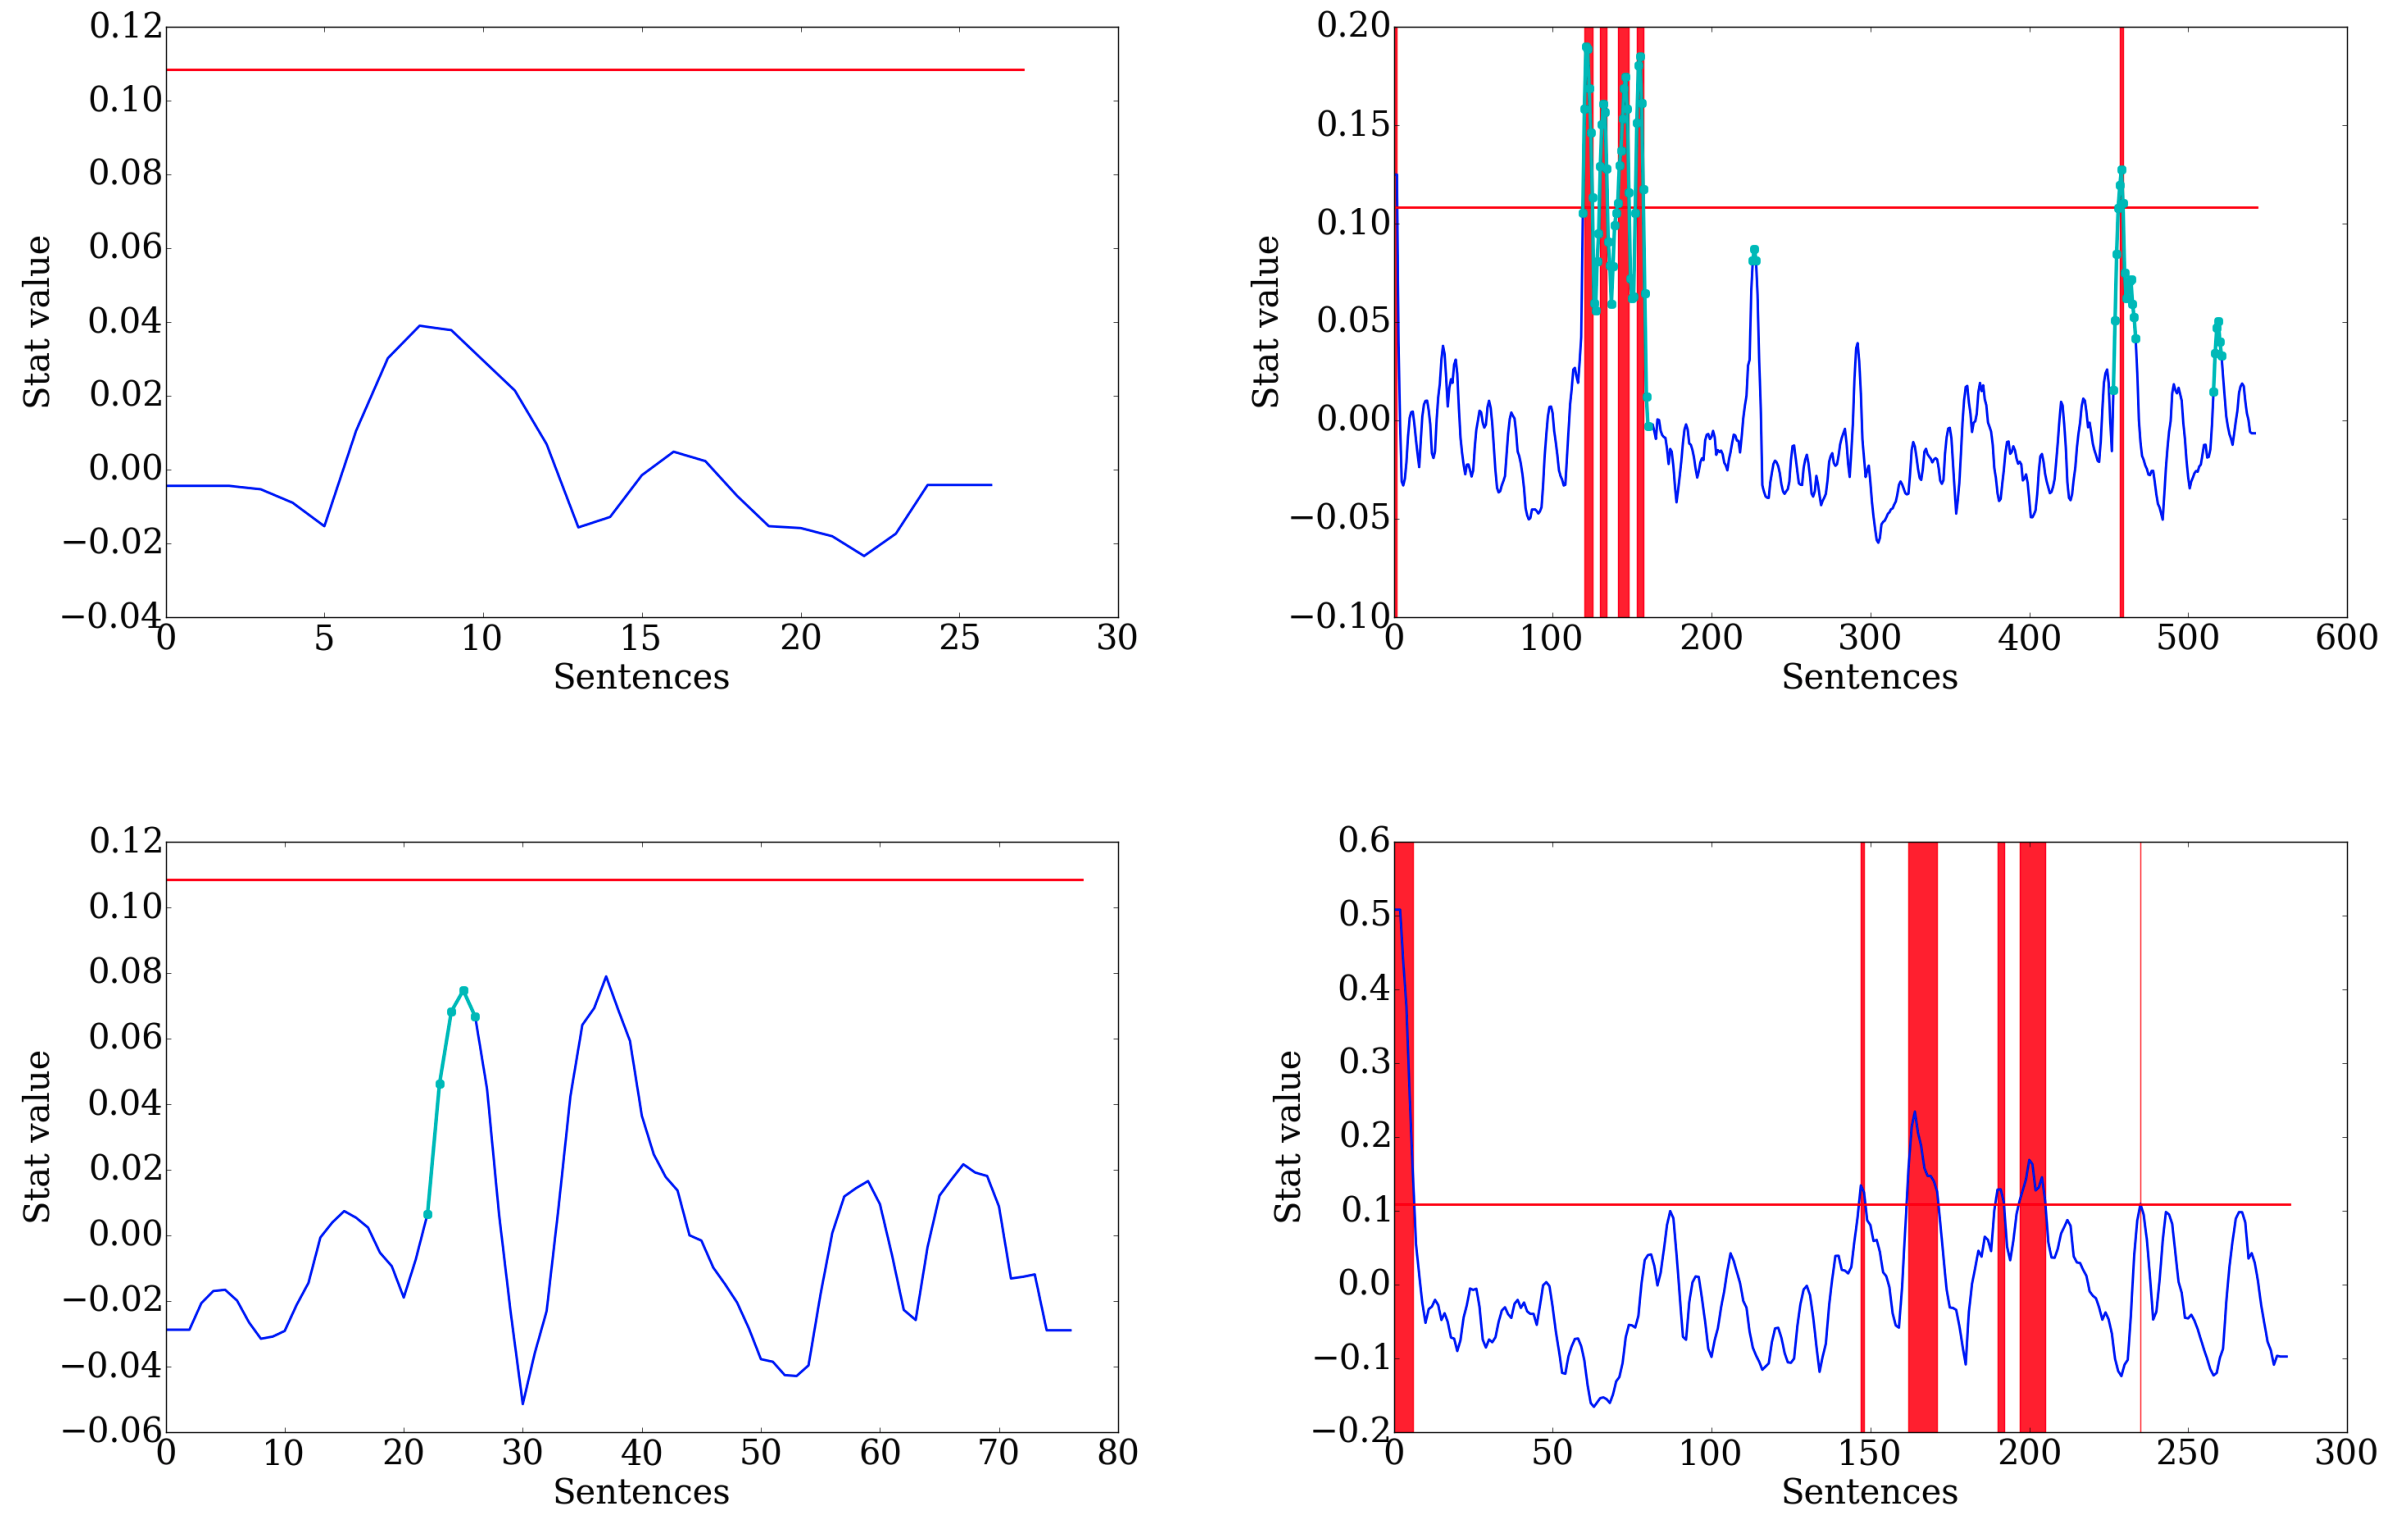
\includegraphics[scale=.26]{clef_text_as_time_series}\\
\centering{Plagiarism detection examples}

\end{frame}
%=============================================
\begin{frame}{Appendix: text data as time series, illustration (2)}

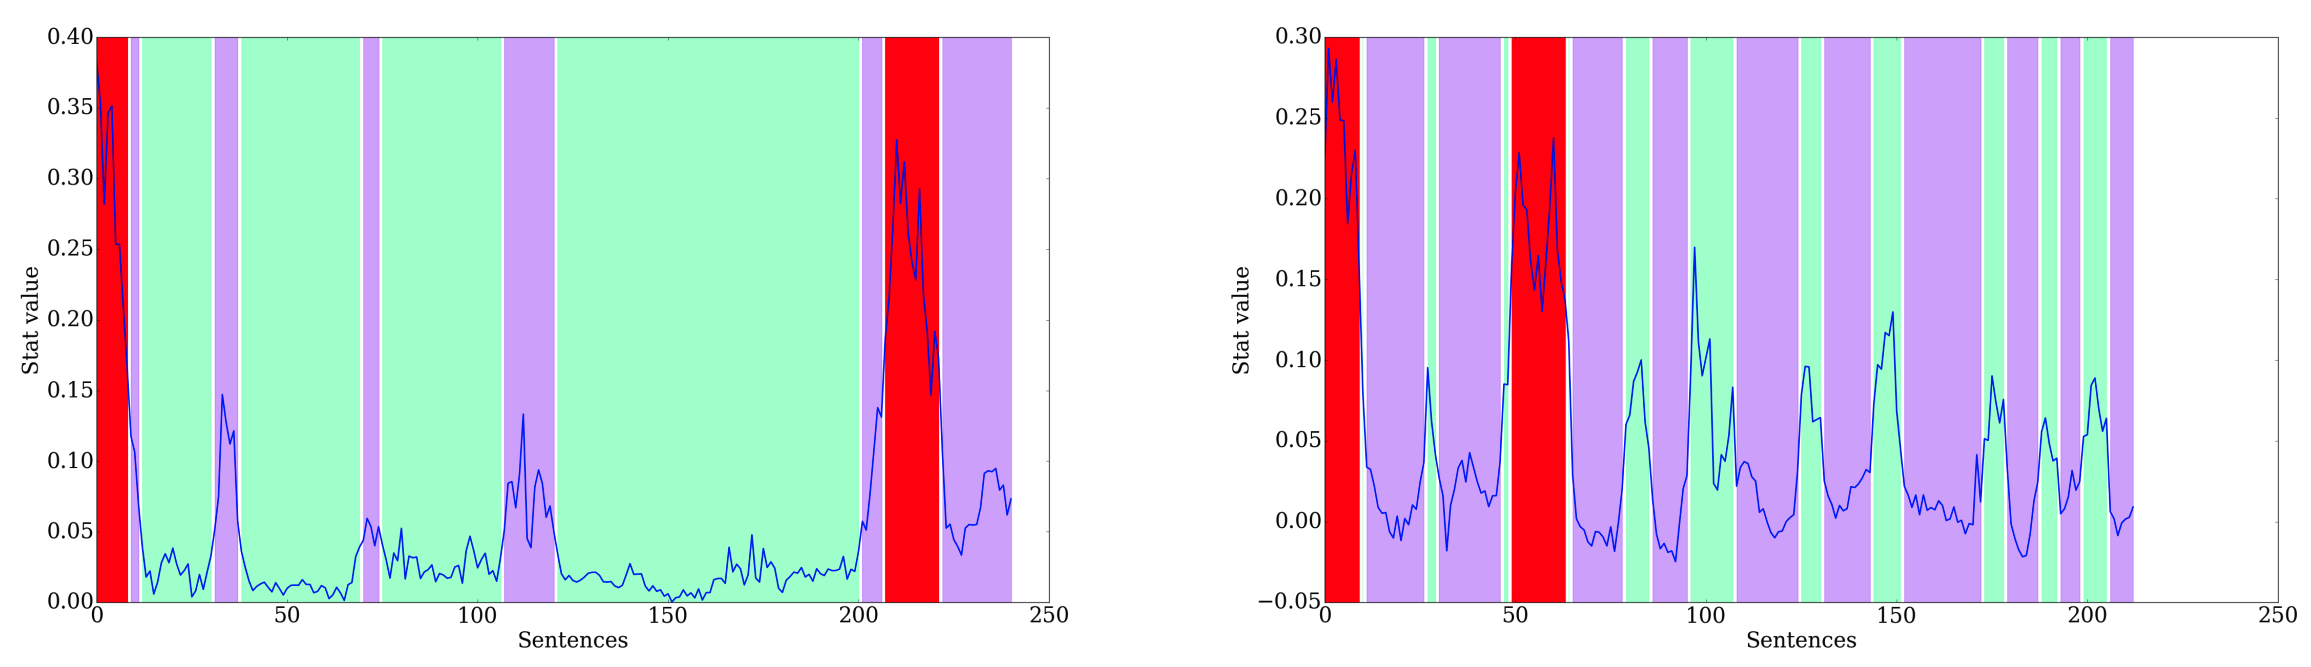
\includegraphics[scale=.27]{clef_text_segmentation}\\
\centering{Text segmentation markdown}

\end{frame}
%=============================================
\begin{frame}{Appendix: phase trajectory of time series}

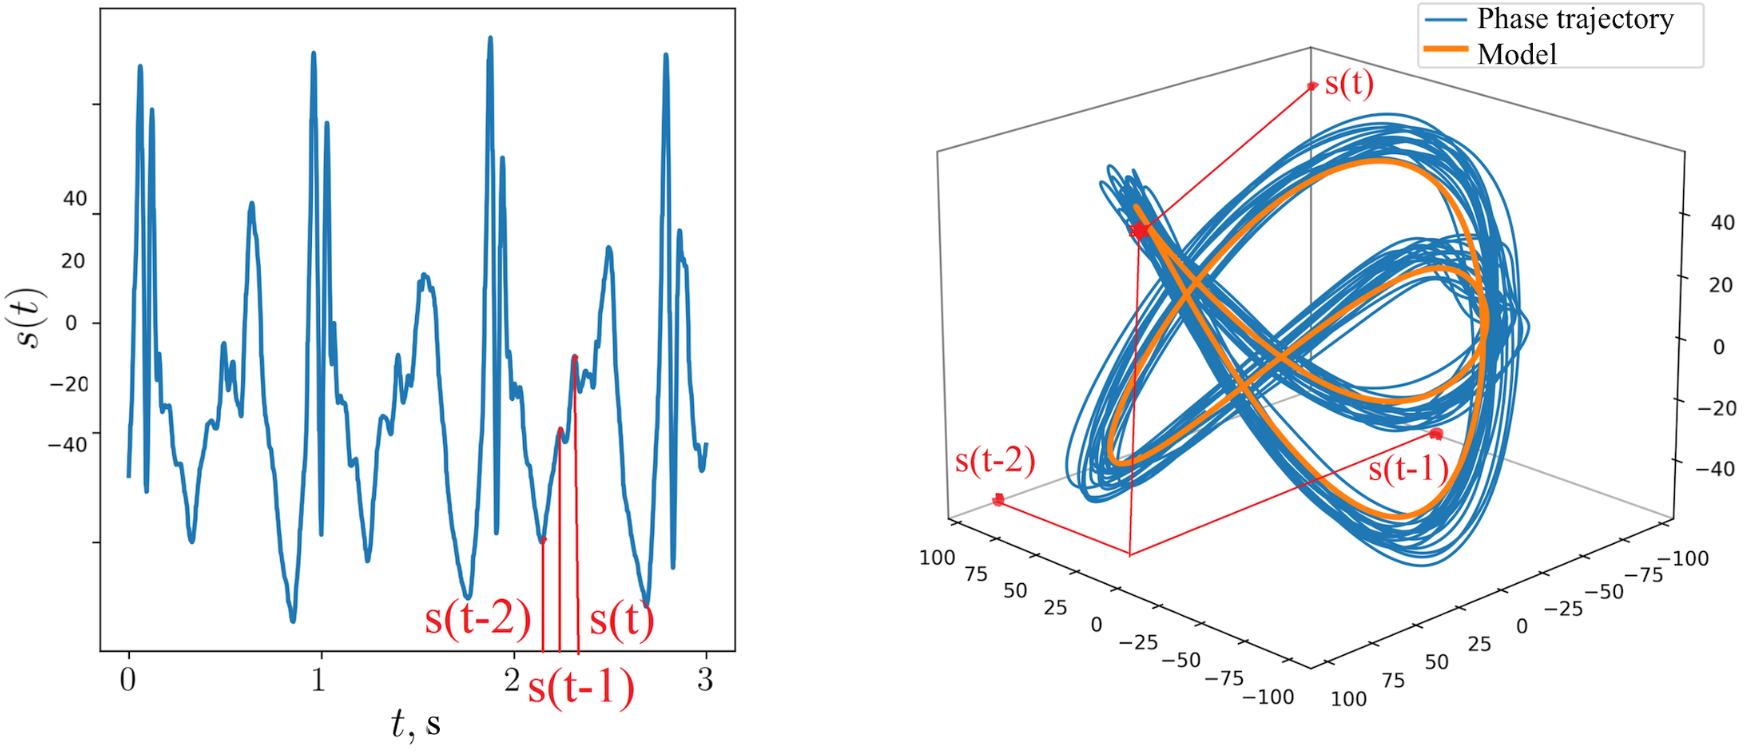
\includegraphics[scale=.37]{phase_trajectory_dimensionality}\\
\centering{Delay embedding delivers dimensionality reduction and keeps the reconstruction}

\end{frame}
%=============================================
\begin{frame}{Appendix: convergent cross-mapping}

{\centering{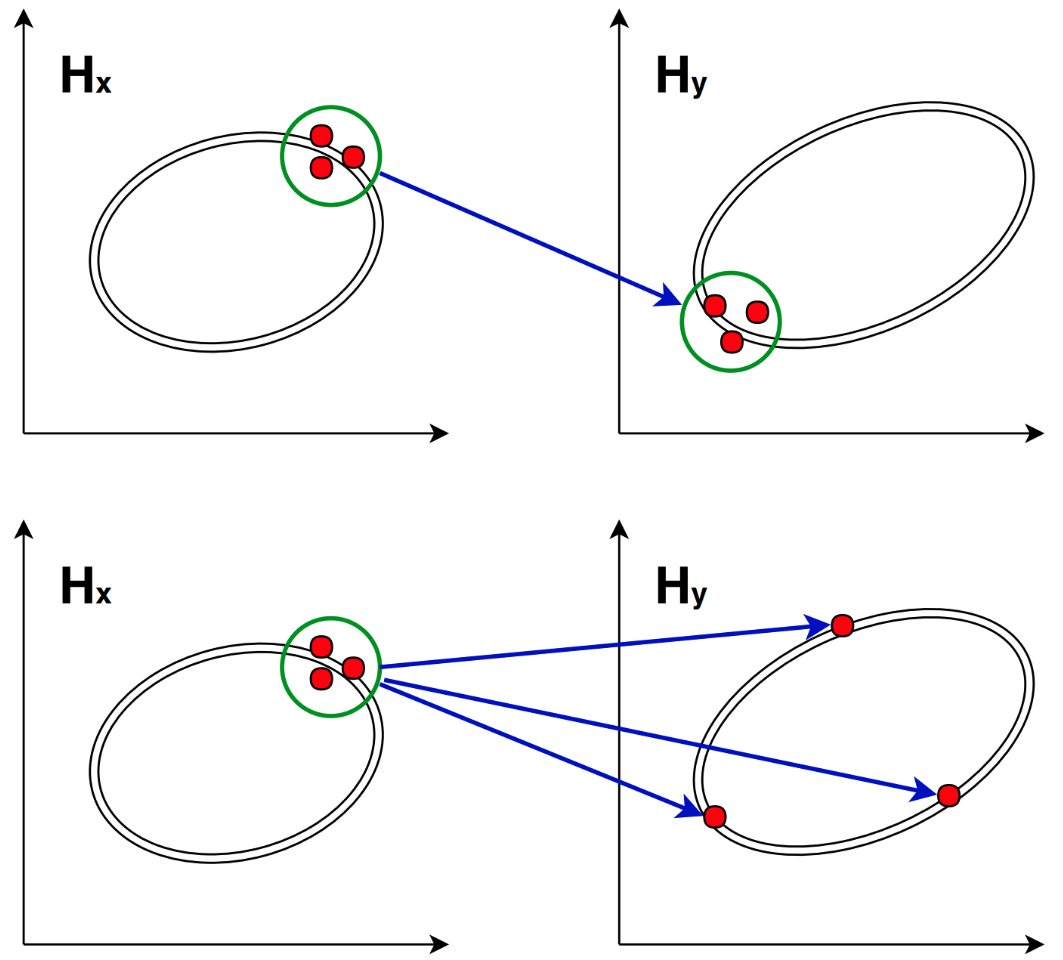
\includegraphics[scale=.35]{convergent_cross-mapping}}\\
\centering{The time series $y$ depends on the time series $x$, but not vice versus}}\\

\bigskip
The time series $y$ depends on the time series $x$, if in the
neighbourhood $(x,x^\prime) \in H_x$ there exists a \emph{Lipschitz continuous map}
$\varphi H_x \to H_y$  such that  $\rho\bigl(H_y (\varphi(x,x^\prime)\bigr) \geqslant L \rho H_x (x,x^\prime)$.

\end{frame}






The following hypothesis apply for each set:
1. The system state is reconstructable, so there is a pair P,Q and Err for both
2. There is a noise is independent between two sets
3. Variant 1 there is a common basis
4. Variant 2 we need alignment with
5. There is a basis in both spaces and there is a dependency as a
6. bipartite graph
7. triangular graph





%=============================================
\end{document}

\begin{frame}{Delay Embedding}

A time series $\{x_i\}_1^N$ is an array of $N$ numbers
\begin{itemize}
    \item representing the values of some measured (observed) dynamical variable $\mathbf{x}(t)$,
    \item taken at a constant time step $\Delta t$.
\end{itemize}

Often, it is convenient to represent a time series in the form of \textit{phase trajectories} — instead of using the variables of the system directly, we use delay vectors:
$$ \mathbf{z}_i = [x_i, x_{i-1}, \dots, x_{i-m+1}]. $$
Each such vector is an element of the $m$-dimensional phase space $\mathbb{R}^m$.
\end{frame}
%=============================================
\begin{frame}{Elements of Takens' Theory}

\begin{itemize}
    \item Let a dynamical system $f(\mathbf{x})$ be given with phase space $\mathbb{R}^M$.
    \item The quantities forming the time series are the values of some function $h$ of the state $\mathbf{x}(t)$ of this dynamical system on a manifold $W^d \subset \mathbb{R}^M$:
    $$ h: W^d \rightarrow \mathbb{R}, \qquad x_i = h(\mathbf{x}(t_i)) = h(f(\mathbf{x}_0, t_i)). $$
    \item With a fixed time step $\Delta t$:
    $$ \mathbf{x}(t) = f(\mathbf{x}_0, t_i + i \cdot \Delta t). $$
\end{itemize}

Therefore, for the components of the delay vectors we have:

$$ x_i = h(\mathbf{x}(t_i)) = h(f(\mathbf{x}_0,t_i)) $$
$$ x_{i+1} = h(\mathbf{x}(t_{i+1})) = h(f(\mathbf{x}_0, t_i + \Delta t)) $$
$$ \dots $$
$$ x_{i+m-1} = h(\mathbf{x}(t_{i+m-1})) = h(f(\mathbf{x}_0, t_i + (m-1)\cdot \Delta t)) $$

\end{frame}

%=============================================
\begin{frame}{Elements of Takens' Theory}

Since all components of the vector
$$\mathbf{z}_i = [x_i, x_{i-1}, \dots, x_{i+m-1}]$$
can be associated with the same measurement of the dynamical system's state
$$x_i = h(f(\mathbf{x}_0, t_i)),$$
there exists a vector-valued function $\Lambda$ that maps $x_i$ into vectors in the $m$-dimensional space $\mathbb{R}^m$:

$$
\mathbf{z}_i = \Lambda(x_i), \qquad \mathbf{z}_i \in \mathbb{R}^m.
$$

These considerations form the core of Takens' theorem, which states that when
$$ m \geq 2d + 1, $$
the mapping $\Lambda$ constitutes an embedding of the manifold $W^d$ into $\mathbb{R}^m$.

\end{frame}
%=============================================



\end{document}
